\documentclass{article}
\usepackage[margin=1.25in]{geometry}
\usepackage{amsmath, amssymb, setspace, enumerate, enumitem}
\usepackage{enumerate}
\usepackage{setspace}
\usepackage{graphicx}
\onehalfspacing

\begin{document}
    \begin{enumerate}
        \item Simplify the following expressions using Boolean algebraic laws. Give each step of your simplification and denote which laws you’re using for each step. Do not skip or combine steps!
        \begin{enumerate}
            \item $A \cdot (A + B \cdot B) + (B + A) \cdot (A + B)$\\[0.25in]
            \begin{tabular}{c | c}
                $A \cdot (\overline{A} + BB) + \overline{(B+A)} \cdot (\overline{A} + B)$ & Demorgan's Law\\
                $A \cdot (\overline{A} + BB) + (\overline{B} \cdot \overline{A}) \cdot (\overline{A} + B)$ & Idempotent Law\\
                $A \cdot (\overline{A} + B) + (\overline{B} \cdot \overline{A}) \cdot (\overline{A} + B)$ & Distributive Law\\
                $(\overline{A} + B)(A+\overline{B} \cdot \overline{A})$ & Distributive Law\\
                $(\overline{A} + B)(A + \overline{B} \cdot A + \overline{A})$ & Inverse Law\\
                $(\overline{A} + B)(A + \overline{B} \cdot 1)$ & Identity Law\\
                $(\overline{A} + B)(A + \overline{B})$ & Distributive Law\\
                $(\overline{A} + B)A + (\overline{A} + B)\overline{B}$ & Distributive Law\\
                $A\overline{A} + AB + \overline{A}\cdot\overline{B} + \overline{B}B$ & Inverse Law\\
                $0 + AB + \overline{A}\cdot\overline{B} + 0$ & Identity Law\\
                $AB + \overline{A}\cdot\overline{B} + 0$ & Identity Law\\
                \boldmath{$AB + \overline{A}\cdot\overline{B}$}
            \end{tabular}
            \item $\overline{C \cdot B} + A \cdot B \cdot C + \overline{A + C + \overline{B}}$\\[0.25in]
            \begin{tabular}{c | c}
                $\overline{CB} + ABC + \overline{A + C + \overline{B}}$ & Demorgan's Law\\
                $(\overline{C} + \overline{B}) + ABC + \overline{A + C + \overline{B}}$ & Demorgan's Law\\
                $(\overline{C} + \overline{B}) + ABC + \overline{A} \cdot \overline{C}B$ & Commutative Law\\
                $(\overline{C} + \overline{B}) + ABC + \overline{A} B \overline{C}$ & Absorption Law\\
                \boldmath{$(\overline{C} + \overline{B}) + A$}\\
            \end{tabular}
            \item $(A + B) \cdot (\overline{A} + C) \cdot (\overline{C} + B)$\\[0.25in]
            \begin{tabular}{c | c}
                $(A + B)(\overline{A} + C)(\overline{C} + B)$ & Distributive Law\\
                $(A + B)(\overline{A} + C)\overline{C} + (A+B)(\overline{A} + C)B$ & Distributive Law\\
                $(A+B)(\overline{A} \cdot \overline{C}) + (A+B)(C \overline{C}) + (A+B)(\overline{A} + C)B$ & Inverse Law\\
                $(A+B)(\overline{A} \cdot \overline{C}) + (A+B)(0) + (A+B)(\overline{A} + C)B$ & Zero and One Law\\
                $(A+B)(\overline{A} \cdot \overline{C}) + (A+B) (\overline{A} + C)B$ & Distributive Law\\
                $(A+B)(\overline{A} \cdot \overline{C}) + (\overline{A} + C)(AB) + (\overline{A} + C)(BB)$ & Idempotent Law\\
                $(A+B)(\overline{A} \cdot \overline{C}) + (\overline{A} + C)(AB) + (\overline{A} + C)(B)$ & Distributive Law\\
                $A\overline{A} \cdot \overline{C} + \overline{A}B\overline{C} + (\overline{A} + C)(AB) + (\overline{A} + C)(B)$ & Inverse Law\\
                $0\overline{C} + \overline{A}B\overline{C} + (\overline{A} + C)(AB) + (\overline{A} + C)B$ & Zero and One Law\\
                $\overline{A}B\overline{C} + (\overline{A} + C)(AB) + (\overline{A} + C)B$ & Distributive Law\\
                $\overline{A}B\overline{C} + \overline{A}AB + ABC + (\overline{A} + C)B$ & Inverse Law\\
                $\overline{A}B\overline{C} + 0B + ABC + (\overline{A} + C)B$ & Zero and One Law\\
                $\overline{A}B\overline{C} + ABC + (\overline{A} + C)B$ & Distributive Law\\
                $\overline{A}B\overline{C} + ABC + \overline{A}B + BC$ & Commutative Law\\
                $\overline{A}B + BC + ABC + \overline{A}B\overline{C}$ & Absorption Law\\
                \boldmath{$\overline{A}B + BC$}\\
            \end{tabular}
        \end{enumerate}
        \item Find all solutions of the following Boolean equations without using the truth tables:
        \begin{enumerate}
            \item $(\overline{A} + C) \cdot (\overline{B} + D + A) \cdot (D + A \cdot \overline{C}) \cdot (\overline{D} + A) = 1$
            \begin{itemize}
                \item $(\overline{A} + C)(\overline{B} + D + A)(D + A\overline{C})(\overline{D} + A) = 1$
                \item $(\overline{A} \cdot \overline{B} + \overline{A}D + \overline{A}A + C\overline{B} + CD + AC)(D + A\overline{C})(\overline{D} + A) = 1$
                \item $(A\overline{B} + \overline{A}D + C\overline{B} + CD + AC)(D + A\overline{C})(\overline{D} + A) = 1$
                \item $(A\overline{B}D + \overline{A}DD + C\overline{B}D + CDD + ACD + A\overline{B}A\overline{C} + \overline{A}DA\overline{C} + C\overline{B}A\overline{C} + CDA\overline{C} + ACA\overline{C})(\overline{D}+A) = 1$
                \item $(A\overline{B}D + \overline{A}D + C\overline{B}D + CD + ACD + A\overline{B} \cdot \overline{C})(\overline{D} + A) = 1$
                \item $(A\overline{B}D\overline{D} + \overline{A}D\overline{D} + C\overline{B}D\overline{D} + CD\overline{D} + ACD\overline{D} + A\overline{B}\cdot \overline{C} \cdot \overline{D} + AA\overline{B}D + \overline{A}AD + AC\overline{B}D + ACD + AACD + AA\overline{B}\cdot \overline{C} = 1$
                \item $A\overline{B} \cdot \overline{C} \cdot \overline{D} + A\overline{B}D + AC\overline{B}D + ACD + ACD + A\overline{B} \cdot \overline{C} = 1$
                \item $A\overline{B} \cdot \overline{C} \cdot \overline{D} + A\overline{B}D + AC\overline{B}D + ACD + A\overline{B} \cdot \overline{C} = 1$
                \item $\overline{B}(A\overline{C}D + AD + ACD + A\overline{C}) + ACD = 1$
                \item $\overline{B}(ACD) + ACD = 1$
            \end{itemize}
            \begin{center}
                \textbf{The equation is true when ALL of $ACD$ is true, or $ACD = 1$}
            \end{center}
            \item $(((\overline{K} \cdot L \cdot N) \cdot (L+M)) + ((\overline{K} + L + N) \cdot (K \cdot \overline{L} \cdot \overline{M}))) \cdot (\overline{K} + \overline{N}) = 1$
            \begin{itemize}
                \item $(\overline{K}LNL + \overline{K}LNM + K\overline{L}M\overline{K} + K\overline{L}L\overline{M} + K\overline{L}N\overline{M})(\overline{K} + \overline{N}) = 1$
                \item $(\overline{K}LN + \overline{K}LNM + K\overline{L}N\overline{M})(\overline{K} + \overline{N}) = 1$
                \item $\overline{K}\cdot\overline{K}LN + \overline{K}LNM\overline{K} + K\overline{K}\cdot\overline{L}\cdot\overline{M}N + \overline{K}LN\overline{N} + KLNM\overline{N} + K\overline{L}MN\overline{N} = 1$
                \item $\overline{K}LN+\overline{K}LNM=1$
                \item $\overline{K}(LN + LNM) = 1$
                \item $\overline{K}(LN) = 1$
                \item $\overline{K}LN = 1$
            \end{itemize}
            \begin{center}
                \textbf{The equation is true when $LN$ is true and $K$ is false, or $\overline{K}LN = 1$}
            \end{center}
        \end{enumerate}
        \item Simplify the following expression by first constructing a truth table, using that truth table to construct a K-map, and then using that K-map to simplify.\\
        $Q = \overline{X} \cdot \overline{Y} \cdot Z + X \cdot Y \cdot \overline{Z} + \overline{X} \cdot Y \cdot \overline{Z} + X \cdot \overline{Y} \cdot \overline{Z}$\\[0.25in]
        \begin{tabular}{c | c | c | c}
            x & y & z & result\\
            0 & 0 & 0 & T\\
            0 & 0 & 1 & F\\
            0 & 1 & 0 & T\\
            0 & 1 & 1 & F\\
            1 & 0 & 0 & T\\
            1 & 0 & 1 & F\\
            1 & 1 & 0 & T\\
            1 & 1 & 1 & F\\
        \end{tabular}\\[0.25in]
        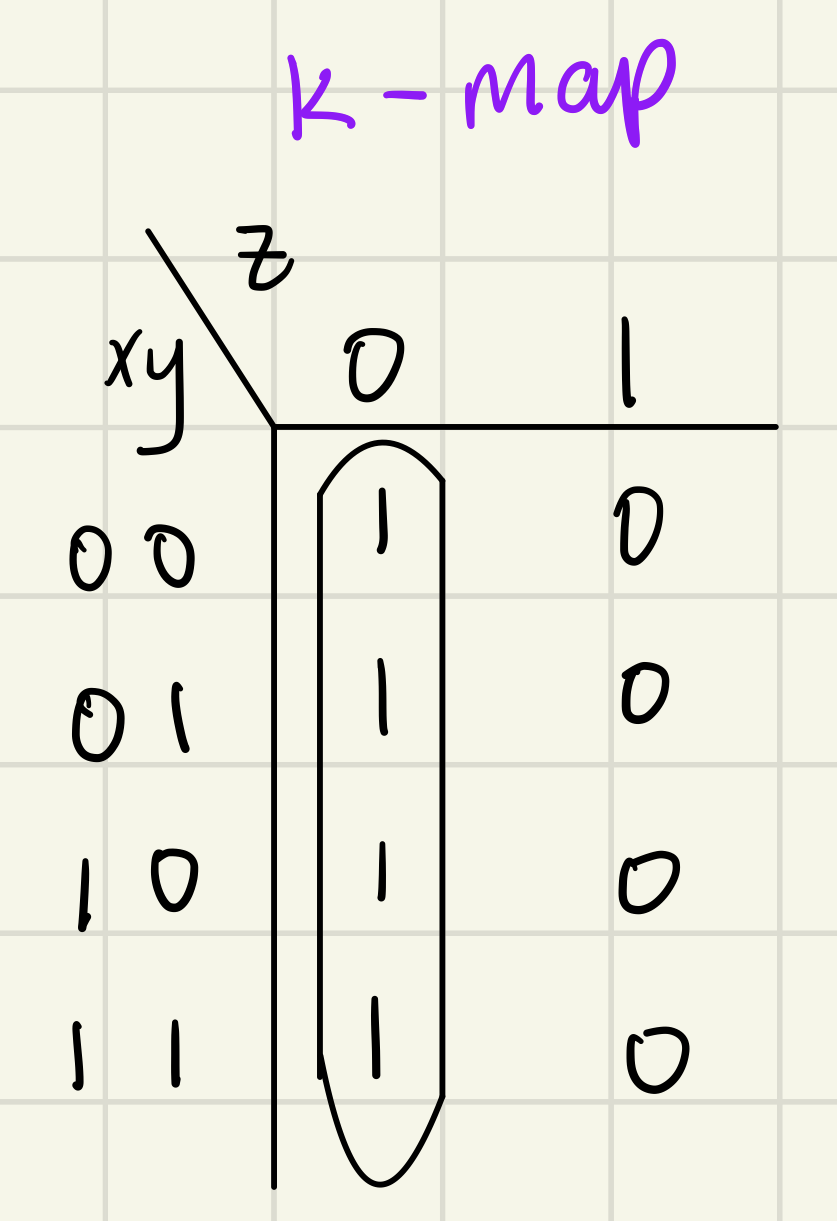
\includegraphics[width=50mm,scale=0.5]{q3_kmap.png}
        \begin{center}
            \textbf{This k-map simplifies the equation to $\overline{Z}$}
        \end{center}
        \item Convert the following truth table into its sum of products representation:\\[0.25in]
        \begin{tabular}{c c c | c}
            A & B & C & Output\\
            0 & 0 & 0 & 1\\
            0 & 0 & 1 & 0\\
            0 & 1 & 0 & 1\\
            0 & 1 & 1 & 1\\
            1 & 0 & 0 & 0\\
            1 & 0 & 1 & 0\\
            1 & 1 & 0 & 0\\
            1 & 1 & 1 & 1\\
        \end{tabular}
        \begin{itemize}
            \item Sums of product: $\overline{A} \cdot \overline{B} \cdot \overline{C} + \overline{A}B\overline{C} + \overline{A}BC + ABC$
            \item $\overline{A} \cdot \overline{C} (\overline{B} + B) + BC(\overline{A} + A)$
            \item $\overline{A} \cdot \overline{C} 1 + BC 1$
            \item \textbf{Simplified version:} \boldmath{$\overline{A} \cdot \overline{C} + BC$}
        \end{itemize}
        \item Draw a logical circuit diagram that represents the above sum of products expression
        using OpenCircuits (https://opencircuits.io/). Clearly label all inputs/outputs and all
        components. Make sure you connect appropriate input components (e.g., buttons, switches,
        clocks, etc.) and output components (e.g., LEDs, displays, etc.) to facilitate testing of
        your circuit. Download your diagram using OpenCircuits’ “Download” feature, rename it to
        hw4\_SOP.circuit, and submit on Submitty along with your hw4.pdf file.
        \begin{center}
            \textbf{The answer to this question is in file hw4\_SOP.circuit.}
        \end{center}
        \item Test you circuit by supplying appropriate inputs and observing the expected values of the
        output. Explain why your set of tests is sufficient to prove that your logical circuit does in
        fact implement the required Boolean function. For each test, provide a picture (snapshot) of
        your circuit. Insert all such pictures in the hw4.pdf PDF file. You can download pictures
        (PNG, JPEG, or PDF) of your circuit diagram using OpenCircuits’ “Export Image” feature.
        \begin{center}
            \textbf{The images of the circuit diagram is submitted as A\_B\_C.png}\\[0.25in]
            \textbf{0\_0\_0.png is true as seen in the truth table, the LED light is on}\\
            \textbf{0\_1\_0.png is true as seen in the truth table, the LED light is on}\\
            \textbf{0\_1\_1.png is true as seen in the truth table, the LED light is on}\\
            \textbf{1\_1\_1.png is true as seen in the truth table, the LED light is on}\\
            \textbf{0\_0\_1.png is false as seen in the truth table, the LED light is off}\\
            \textbf{1\_0\_0.png is false as seen in the truth table, the LED light is off}\\
            \textbf{1\_0\_1.png is false as seen in the truth table, the LED light is off}\\
            \textbf{1\_1\_0.png is false as seen in the truth table, the LED light is off}\\
        \end{center}
        \item Given inputs A and B, show that NOR {(A + B)} is functionally complete by giving logical
        circuits equivalent to AND {(A * B)}, OR {(A + B)}, and NOT {A} gates using only NOR
        gates in their construction.
        \begin{center}
            \textbf{NOR\_and.circuit represents AND}\\
            \textbf{NOR\_or.circuit represents OR}\\
            \textbf{NOR\_not.circuit represents NOT}
        \end{center}
        \item Hi
    \end{enumerate}
\end{document}